\documentclass{picocon-fanzine}
\usepackage{xcolor}
\usepackage{soul}
\usepackage{array}
\usepackage{textgreek}
\usepackage{pgfplots}
\usepackage{pgfplotstable}
\usepackage{xcolor}
\usepackage{soul}
\usepackage{amsmath}
\usepackage{pdfpages}
\usepackage{eso-pic}

\renewcommand{\tombstone}{%
  
\includegraphics[height=\fontcharht\font`\B,clip]{img/tombstone}%
}

\begin{document}
% \thispagestyle{empty}
% % 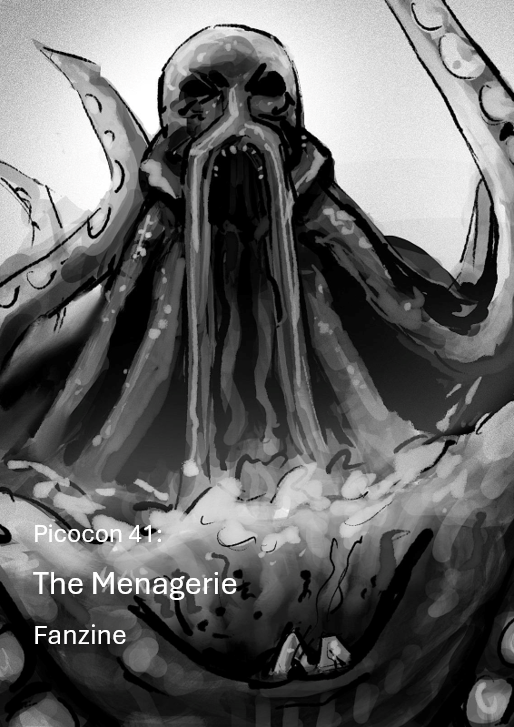
\includepdf{img/fanzine-41-cover-previs.png}
% \text{ }
% \clearpage
\begin{titlepage}
    \AddToShipoutPictureBG*{%
              \AtPageLowerLeft{%
                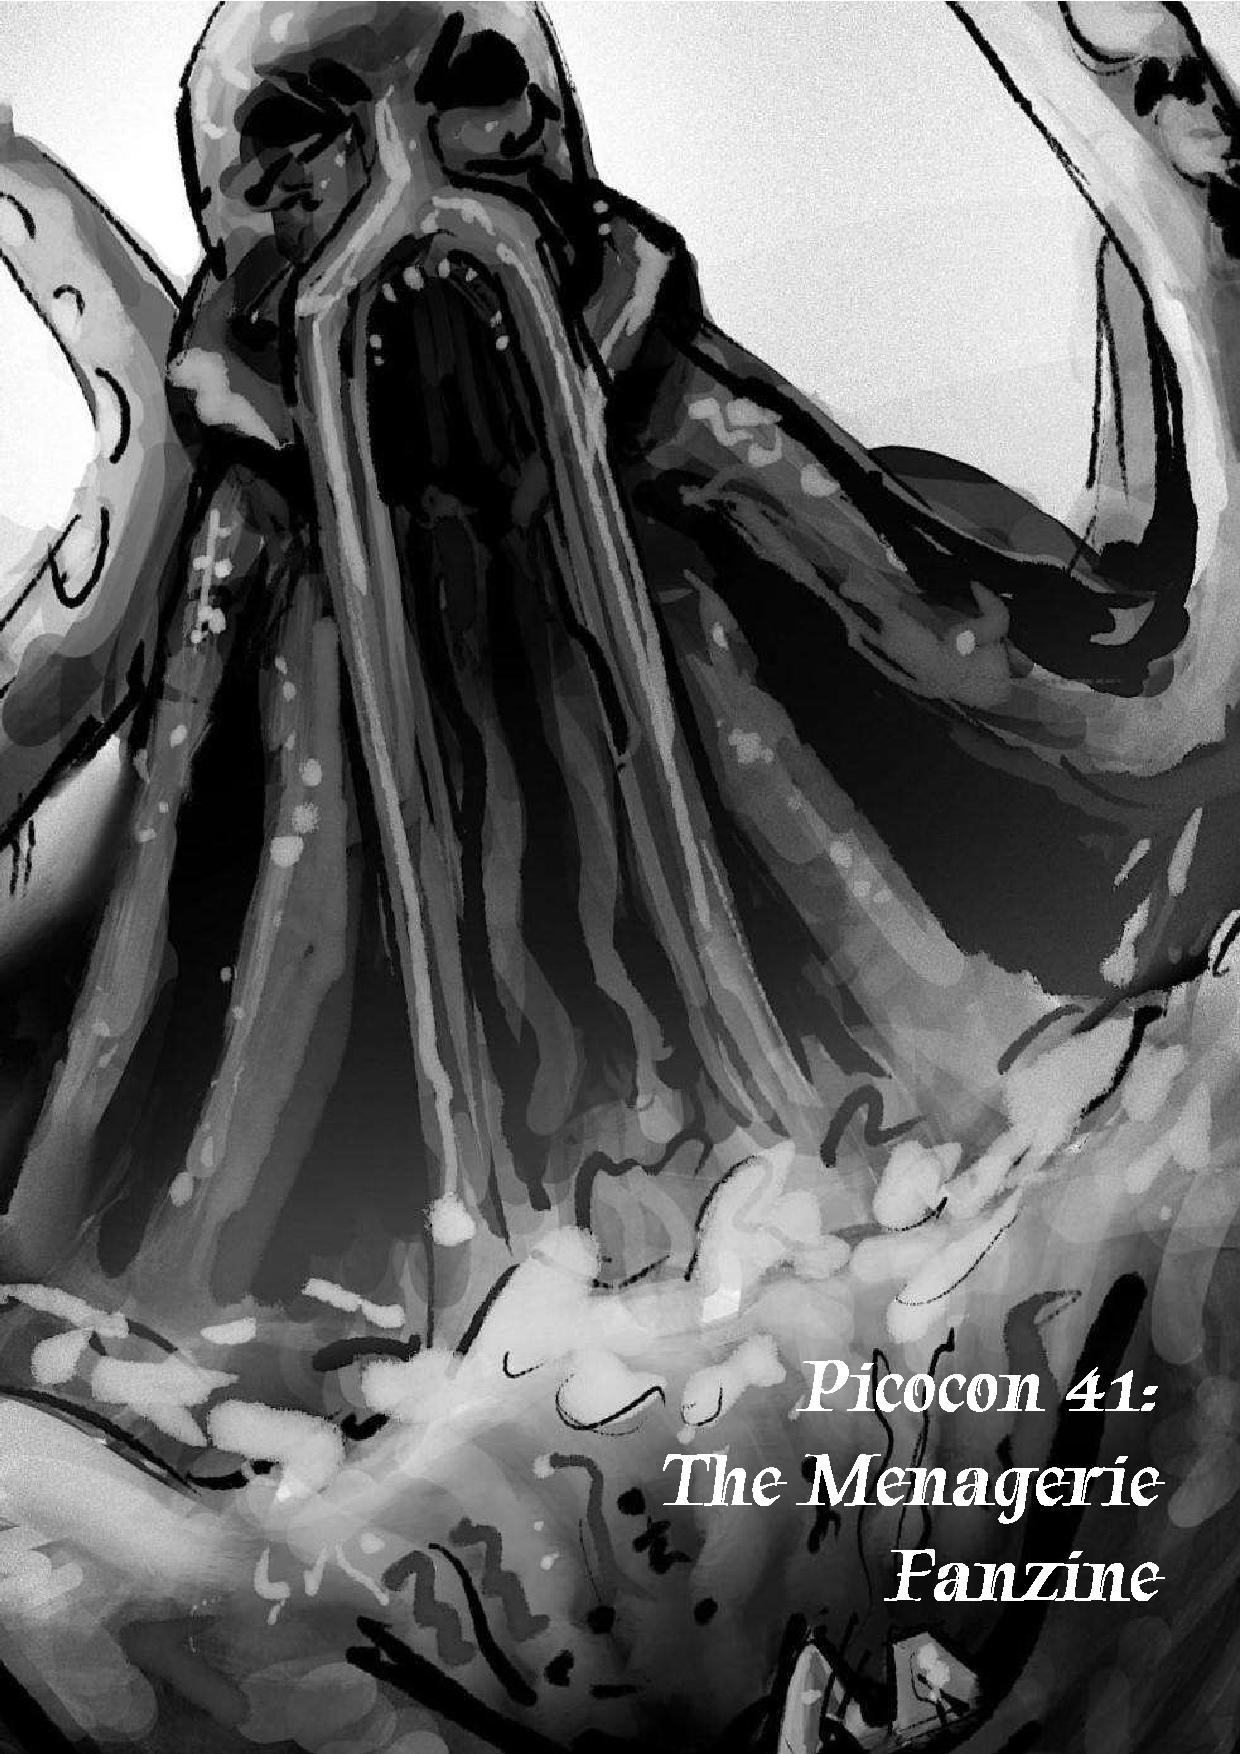
\includegraphics[width=\paperwidth,height=\paperheight]{img/fanzine-cover.pdf}%
              }%
            }
            \vspace*{20cm}
            \color{white}
            % \fontfamily{ntxtlf}\selectfont % Times New Roman font
            % default lmvtt (Latin Modern Typewriter)
            \fontsize{25}{48}\selectfont 
            % Picocon 41:\\ 
            % \fontsize{35}{48}\selectfont The Menagerie \\ 
            % \fontsize{30}{48}\selectfont Fanzine
            % \centering{
            %     {\fontsize{40}{48}\selectfont 
            %     A book title}
            % }\\
            % \vspace{10mm}
            % \centering{\Large{AAAA}}\\
            % \vspace{\fill}
            % \centering \large{BBB}
\end{titlepage}
\begin{center}
    % \vspace*{10cm}
    \normalfont \textbf{Kraky} \textemdash{} cover page by Hetty Symes
\end{center}
\pagenumbering{roman}
\setcounter{page}{1}
\clearpage
\pagenumbering{arabic}
\setcounter{page}{1}
\head{From the Editor}
% Thank you, Luke (also hi new editor here), and we return all the love to those who sent us their wonderfully twisty work to this fanzine. For those of you who've been handed this humble collection, be sure to check out the Picocon \emph{Wyrmtongue} to find out what's happening, and most of all, enjoy the convention!
\noindent Hello again, fellow nerds, to another edition of the Picocon Fanzine! This year, we have tales of magic and monsters, and wonderful artwork of Lovecraftian horrors. One might call it a bona fide \textit{menagerie}\footnote{Honestly who made this guy editor}! Thanks again to our incredibly talented (and busy!) friends at Imperial who made something to keep this collection alive, and special thanks to Hetty Symes for the amazing cover page. This literally could not have happened without all of your help. 

As always, be sure to check out the Picocon \textit{Wyrmtongue} to find out what's happening, and remember, ENJOY!
\tombstone

\hfill \parbox{0.5\textwidth}{{\large\textbf{\textemdash{} Clifford Chan - Lord of Words}}\\\hspace*{1.7em}March 2024}
\vfill

\tableofcontents
\vfill
\clearpage

% \story{Rumpelstiltskin}{Rebecca Allday}{A twisted retelling of a classic fairytale}{txt/rebecca-a}
% \vspace{50px}

% \begin{center}
% 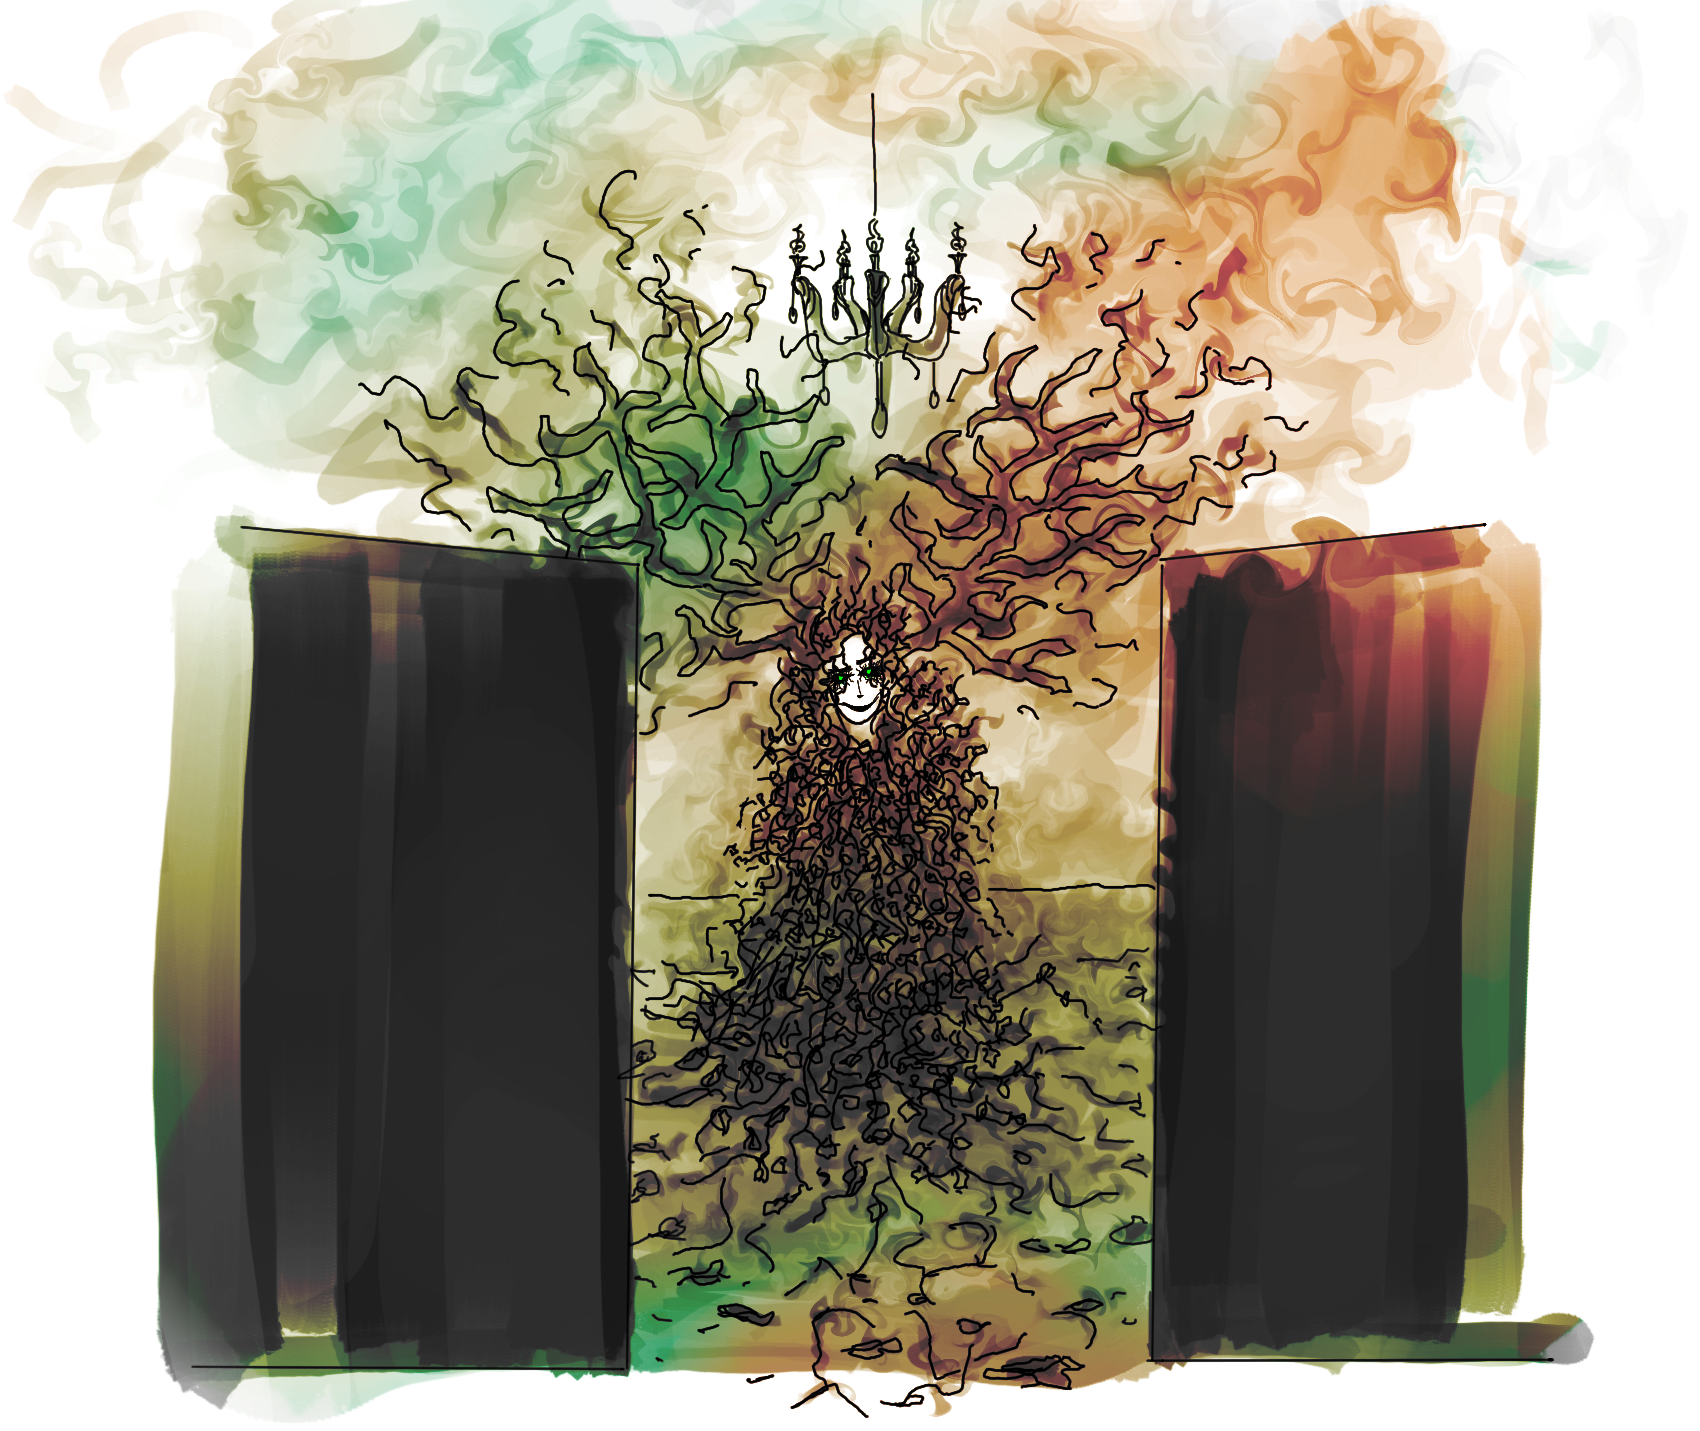
\includegraphics[width=1\textwidth]{img/rumplestiltskin.png}
% \end{center}

% \centerline{\emph{Illustration by Rebecca Allday}}
% \vfill
\story{Leave No Trace}{Juairiyah Raqib}{A team of human colonists explore an alien planet.}{txt/riyah-story}
\vfill
\clearpage

\poem{Kingmaker}{Aditi Mehendale}{txt/kingmaker}
\vfill
\clearpage

\artpage{The Lady of Bloom}{Rebecca Allday}{img/the-lady-of-bloom-cropped}
\vfill
\clearpage

\story{The League of Femmes Fatales}{Clifford Chan}{The League of Femmes Fatales gather to discuss their plans for world domination.}{txt/league-of-femmes-fatales}
\vfill
\clearpage

\story{Real Wizards FM}{Lucas S Schuck}{Real wizards drive or die.}{txt/real-wizards-fm}
\vfill
\clearpage

\story{A Ball of Midnight}{Anand Doshi}{}{txt/a-ball-of-midnight}
\vfill
\clearpage

\story{The Spiders that Eat You}{Kai Lam}{}{txt/the-spiders-that-eat-you}
\vfill
\clearpage

\text{ }
\clearpage

\clearpage
\thispagestyle{empty}
\vspace*{\fill}
\begin{center}
  
\includegraphics[width=0.5\textwidth]{img/icsf-logo}
\end{center}
\vspace{4em}
\end{document}
